 %GPL V3 by Mathias Hablützel, feel free to improve this template
 \documentclass[a4paper,10pt]{article}
 
 % Use UTF8 since the laptop is configured so and use ngerman for word breaking.
 % If you encounter an encoding problem, remove the line with utf8.
 \usepackage[utf8]{inputenc}
 \usepackage[ngerman]{babel}
 \usepackage[pdftex]{graphicx}
 
 % TikZ für schöne Grafiken und so.
 \usepackage{tikz}
 \usetikzlibrary{positioning,calc,fadings,decorations.pathreplacing,arrows}
 \usepackage{pgfplots}

% \usepackage{hyperref}
 \usepackage{colortbl}
 \usepackage{tabularx}
 \usepackage{color}
 \usepackage{amsfonts}
 \usepackage{amsmath}
 \usepackage{listings}
 \usepackage{multirow}
\usepackage{fancyhdr}
 \usepackage{multicol}
 \usepackage{pdfpages}
 \usepackage[colorlinks=true,
  linkcolor=black,
  citecolor=black,
  filecolor=black,
  pagecolor=black,
  urlcolor=black,
  bookmarks=true,
  bookmarksopen=true,
  bookmarksopenlevel=3,
  plainpages=false,
  pdfpagelabels=true]{hyperref}

% Hack for german umlaute
\lstset{
  literate={ö}{{\"o}}1
           {ä}{{\"a}}1
           {ü}{{\"u}}1
}

% define colors
 \definecolor{hellgrau}{rgb}{0.8,0.8,0.8}

  % http://stackoverflow.com/questions/741985/latex-source-code-listing-like-in-professional-books
  \usepackage{listings}
  \usepackage{courier}
 \lstset{
         basicstyle=\footnotesize\ttfamily, % Standardschrift
         numbers=left,               % Ort der Zeilennummern
         numberstyle=\tiny,          % Stil der Zeilennummern
         stepnumber=1,               % Abstand zwischen den Zeilennummern
         numbersep=5pt,              % Abstand der Nummern zum Text
         tabsize=2,                  % Groesse von Tabs
         extendedchars=true,         %
         breaklines=true,            % Zeilen werden Umgebrochen
         keywordstyle=\color{red},
    		frame=b,         
 %        keywordstyle=[1]\textbf,    % Stil der Keywords
 %        keywordstyle=[2]\textbf,    %
 %        keywordstyle=[3]\textbf,    %
 %        keywordstyle=[4]\textbf,   \sqrt{\sqrt{}} %
         stringstyle=\color{white}\ttfamily, % Farbe der String
         showspaces=false,           % Leerzeichen anzeigen ?
         showtabs=false,             % Tabs anzeigen ?
         xleftmargin=17pt,
         framexleftmargin=17pt,
         framexrightmargin=5pt,
         framexbottommargin=4pt,
         %backgroundcolor=\color{lightgray},
         showstringspaces=false      % Leerzeichen in Strings anzeigen ?        
 }
 \lstloadlanguages{% Check Dokumentation for further languages ...
         %[Visual]Basic
         %Pascal
         %C
         %C++
         %XML
         %HTML
         Java
 }
    %\DeclareCaptionFont{blue}{\color{blue}} 

  %\captionsetup[lstlisting]{singlelinecheck=false, labelfont={blue}, textfont={blue}}
  \usepackage{caption}
\DeclareCaptionFont{white}{\color{white}}
\DeclareCaptionFormat{listing}{\colorbox[cmyk]{0.43, 0.35, 0.35,0.01}{\parbox{\textwidth}{\hspace{15pt}#1#2#3}}}
\captionsetup[lstlisting]{format=listing,labelfont=white,textfont=white, singlelinecheck=false, margin=0pt, font={bf,footnotesize}}


 % I set here a different sidemargin because the original margin looks not so
 % good for normal documents. Additionally I have to enlarge the textwidth.
 \setlength{\oddsidemargin}{0cm}
 \setlength{\evensidemargin}{0cm}
 \addtolength{\textwidth}{4cm}
\newcolumntype{C}[1]{>{\centering\arraybackslash}m{#1}} 

\begin{document} 
 % Here I use the up-to-date font encoding T1 and the font familly Computer Modern
 % Sans Serif (since I don't like the standard font) medium and normal (non-italic or so).
 \usefont{T1}{cmss}{m}{n}

\pagestyle{fancy} %eigener Seitenstil
\fancyhf{} %alle Kopf- und Fußzeilenfelder bereinigen
\fancyhead[C]{LakeRouting - Optimale Wegfindung anhand von Wettermodellen} %zentrierte Kopfzeile
\renewcommand{\headrulewidth}{0.4pt} 
\fancyfoot[C]{\thepage}

 \title{\begin{flushleft}\vspace*{-3cm}
\includegraphics[keepaspectratio,width=7cm]{img/de-zhaw-cmyk}\end{flushleft} \vspace*{4cm} LakeRouting - Optimale Wegfindung anhand von Wettermodellen }
 \date{\today}
 \author{Fevzi Yükseldi (yuksefev@students.zhaw.ch)\\
 Mathias Hablützel (hablumat@students.zhaw.ch)\\
 \\
Prof. Dr. Rudolf M. Füchslin (furu@zhaw.ch)\\
Dr. Jacques Ambühl (jacques.ambuehl@meteoschweiz.ch)}
 
 \maketitle
\thispagestyle{empty}
 \newpage
\thispagestyle{empty}
\part*{Management Summary}

\vspace*{2cm}
\setlength{\columnsep}{2cm}
\begin{multicols}{2}

\textbf{\textsc{Deutsch}}
\vspace{1cm}\\

\columnbreak

\textbf{\textsc{English}}
\vspace{1cm}\\

\end{multicols}
\newpage

\cleardoublepage
\begingroup
\pagestyle{empty}
\setcounter{tocdepth}{2}
\tableofcontents
\clearpage
\endgroup
       
\newpage

\setcounter{page}{1} 
\part{Vorwort}
\section{Einleitung}
Zu den klassischen Methoden der mathematischen Entscheidungsvorbereitung gehört die Dynamische Programmierung (DP). Sie ermöglicht die optimale Gestaltung einer Kette sequentieller Entscheidungen aufgrund wettbewerbsrelevanter Randbedingungen (physikalischer oder ökonomischer Natur).\\
...
%Unvollständig

\section{Ziel / Auftrag}
Die vorgeschlagene Bachelorarbeit schlägt eine Anwendung der DP zur Kursbestimmung eines Segelschiffs vor. Aufgrund der mit einem numerischen Modell vorausgesagten Wetterentwicklung und in Anbetracht der Leistungskurve (Polardiagramm) des Schiffes wird dessen optimale Route mittels DP gerechnet. Ähnliche Methoden wurden beim Alinghi Team im Rahmen des Americas Cup verwendet. \\
Weitere Anwendungen der DP zum Thema "energy trading" für erneuerbare Energiequellen sind denkbar und eine Übertragung der Resultate der BA in diesen Bereich werden von MeteoSchweiz angestrebt. \\

Die Bachelorarbeit läuft unter fachlicher Betreuung der MeteoSchweiz (numerische Meteorologie und angewandte Mathematik). Sie besteht darin, zur Lösung des obigen Problems eine in Java geschriebene Applikation der DP zu entwickeln. Sämtliche zu diesem Zweck nötige Algorithmen sind vorhanden und müssen nicht neu entwickelt werden, hingegen müssen bestehende Algorithmen auf an die spezielle Problemsituation angepasst werden. 

\section{Weitere Informationen sowie Danksagung}
Für die professionelle und freundliche Kooperation möchten wir uns an dieser Stelle herzlich bedanken!\\
...

\newpage
\part{Projektplanung}

\section{Projektübersicht}

\subsection{Benötigte Ressourcen}
\begin{itemize}
\item Menschliche Ressourcen \\
Das Projekt wird von 2 Personen für rund 1 Semester mit der Betreuung eines Dozenten gemäss dem Auftrag des Auftraggebers durchgeführt. Auch seitens des Auftraggebers steht ein Betreuer zu Verfügung, den wir bei Unklarheiten ebenfalls kontaktieren können und von dem wir auch die nötigen Unterlagen zugeschickt bekommen. Ausserdem steht auch ein Nebenbetreuer zur Verfügung, der grundsätzlich für IT spezifische Fragen zuständig ist. Es wird davon ausgegangen, dass alle Projektmitglieder durchschnittlich 20 bis 25 Stunden pro Woche am Projekt arbeiten.\\
\item Räume \\
Es werden keine speziellen Räume gebraucht. Aber für eine bessere, verstärkte und erfolgreiche Zusammenarbeit wurde das Zimmer TE616 in der ZHAW-Schulgebäude reserviert. Ausserdem werden einmal die Woche, jeweils am Dienstag, zwei Zimmer der Abteilung Wetterdienst in der MeteoSchweiz-Gebäude benutzt. Jedoch wird das Projekt weitgehend als virtuelle Organisation geführt, das heisst, dass der physische Standort der Teilnehmer nicht von Bedeutung ist.

\end{itemize}

\subsection{Meetings}
Die Kommunikation im Projekt mit den beiden Betreuer erfolgt in Form von ordentlichen Meetings jeden Dienstag in der Hauptgebäude der MeteoSchweiz in Zürich. Bei Bedarf kann sie auch per E-Mail oder ausserordentlichen Sitzungen stattfinden. Ausserdem wurde für das Projekt 4 Meilensteine definiert, welche dann anstelle der wöchentlichen Sitzungen stattfinden werden. Die Meilensteine liegen bewusst vor dem eigentlichen Abgabetermin, um Pufferzeiten zu schaffen.

\subsection{Kontaktdaten des Auftraggebers}
MeteoSchweiz\\
Eidgenössisches Departement des Innern EDI \\
Bundesamt für Meteorologie und Klimatologie\\
Krähbühlstrasse 58\\
CH-8044 Zürich\\
Tel.   +41 44 256 91 11 \\
Fax   +41 44 256 92 78\\

\section{Vorgehensmodell}
%Unvollständig
Für unser Projekt haben wir uns für das V-Modell entschieden, da die Phasen stabile Anforderungen haben und sie wenig Management-Aufwand benötigen. Desweiteren besitzen sie klare Abgrenzungen und der Umfang der Arbeit ist klar abschätzbar. 

\section{Zeitliche Planung}
%Unvollständig
\subsection{Effektiver Ablauf}
\begin{table}[h!]
\centering 
  \begin{tabular}{| c | l | r | >{\color{red}} r |}
    \hline
    \rowcolor{hellgrau} 
    \textbf{Arbeitspakete} & \textbf{Tasks} & \textbf{Zeitaufwand} & \textbf{\color{black}Effektiv} \\ \hline \hline
    \multirow{1}{*}{} & \textbf{Planung} & \textbf{Tage} & \textbf{Tage}  \\ \cline{2-4} \hline \hline
     & \textbf{Implementierung} & \textbf{Tage} & \textbf{Tage}  \\ \hline
     \multirow{1}{*}{Nr. 1}& Aufgabe 1+2 & 12 Tage & 12 Tage \\ \hline
     Nr. 2 & Aufgabe 3 & 8 Tage & 8 Tage \\ \hline
     Nr. 3& Aufgabe 4 & 8 Tage & 25 Tage \\ \hline
     Nr. 4& Aufgabe 5 & 13 Tage & 10 Tage \\ \hline
     Nr. 5& Aufgabe 6 & 15 Tage &  Tage \\ \hline
     Nr. 6& Aufgabe 7 & 22 Tage &  Tage \\ \cline{2-4}\hline \hline
     Nr. 7& \textbf{Testing / Finetuning} & \textbf{ Tage} & \textbf{ Tage}  \\ \hline \hline
     \multirow{3}{*}{Nr. 8} & \textbf{Erkenntnis} & \textbf{ Tage} & \textbf{ Tage} \\ \cline{2-4}
     & Schlussfolgerung &  Tage &  Tage  \\ \cline{2-4}
     & Arbeitsrevue &  Tage &   Tage \\ \cline{2-4} \hline \hline
     & \textbf{Reserve} & \textbf{10 Tage} & \textbf{ Tage} \\ \hline \hline \hline
     & \textbf{Zeitaufwand insgesamt} & \textbf{ Tage}  & \textbf{ Tage} \\ \hline \hline
  \end{tabular}
  \caption{Projektplan Ablauf}
  \label{EffektivPlan}
\end{table}

\subsubsection{Definition}
1 Tag = 5 Arbeitsstunden pro Person \\

\subsection{Gantt-Diagramm}
\begin{figure}[h!]
\centering
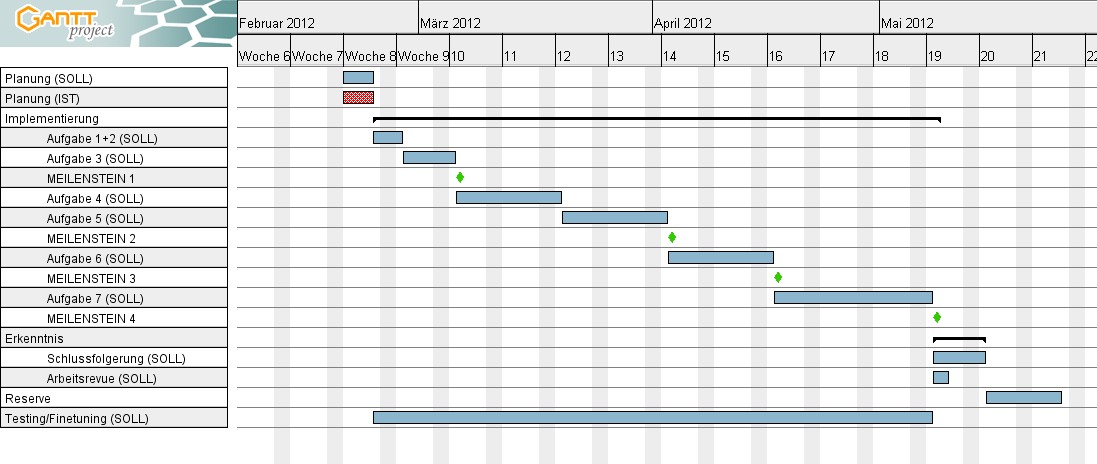
\includegraphics[width=0.8\linewidth]{img/projektplanung.png}
\caption{Projektplan}
\label{prplan}
\end{figure}

\subsection{Arbeitspakete}
Im Folgenden wird das Projekt in Arbeitspakete und ihre Abhängigkeiten eingeteilt, wie es auch in der Tabelle \ref{EffektivPlan} ersichtlich ist. Die Pakete wurden so gewählt, dass sie genau eine geschlossene Aufgabenstellung beschreiben und die Abhängigkeiten definieren, welche Arbeitspakete abgeschlossen sein müssen, damit ein bestimmtes Arbeitspaket begonnen werden kann. Desweiteren wurden auch die geplanten Dauer der Arbeitspakete angegeben. \\

Es ist festgelegt, dass beide Projektmitglieder auch gleichzeitig die Projektleiter für die gesamte Projektlaufzeit sind. Es wird aber im Verlauf des Projektes in jeder einzelnen Phase jeweils ein Projektmitglied die eigentliche Projektleitung übernehmen.
Der Projektleiter der jeweiligen Phase ist hauptverantwortlich für die rechtzeitige Fertigstellung und die Qualität des Produkts der jeweiligen Phase.

\begin{table}[h!]
\centering 
  \begin{tabularx}{\textwidth}{| l | X | l| X | }
    \hline
    \cellcolor{hellgrau}\textbf{Nummer} & \multicolumn{3}{l |}{1}  \\ \hline
    \cellcolor{hellgrau}\textbf{Bezeichnung} & \multicolumn{3}{l |}{Aufgabe 1 \& 2} \\ \hline       
    \cellcolor{hellgrau} & \multicolumn{3}{l |}{•	Erstellung eines Entscheidungsnetzes auf der Erdkugel}  \\ 
    \cellcolor{hellgrau} & \multicolumn{3}{l |}{•	Berechnung einer Orthodromie} \\ 
    \cellcolor{hellgrau} & \multicolumn{3}{l |}{(Distanz in Meilen zwischen zwei Punkten auf der Erdkugel)}  \\ 
    \cellcolor{hellgrau} & \multicolumn{3}{l |}{•	Erstellung der Koordinatendatei eines Sees (in Koordinaten)}  \\ \cline{2-4}
    \cellcolor{hellgrau} & \multicolumn{3}{l |}{•	Erstellung eines Entscheidungskernes in Dynamische Programmierung}  \\ 
     \multirow{-6}{*}{\textbf{\cellcolor{hellgrau}Beschreibung}} & \multicolumn{3}{l |}{•	Berechnung von Orthodromien auf der Erdoberfläche mit Testdaten} \\ \hline
    \cellcolor{hellgrau}\textbf{Start} & 24.02.2012 &  \cellcolor{hellgrau}\textbf{Ende} & 06.03.2012\\ \hline
    \cellcolor{hellgrau}\textbf{Abhängigkeiten} & Keine&  \cellcolor{hellgrau}\textbf{Verantwortung} & Fevzi Yükseldi\\ \hline
  \end{tabularx}
  \caption{Arbeitspaket 1}
\end{table}

\begin{table}[h!]
\centering 
  \begin{tabularx}{\textwidth}{| l | X | l| X | }
    \hline
    \cellcolor{hellgrau}\textbf{Nummer} & \multicolumn{3}{l |}{2}  \\ \hline
    \cellcolor{hellgrau}\textbf{Bezeichnung} & \multicolumn{3}{l |}{Aufgabe 3} \\ \hline       
    \cellcolor{hellgrau} & \multicolumn{3}{l |}{•	Erfassung des Polardiagramms eines Segelschiffes}  \\ 
    \cellcolor{hellgrau} & \multicolumn{3}{l |}{•	Interpolationsverfahren} \\ 
     \multirow{-3}{*}{\textbf{\cellcolor{hellgrau}Beschreibung}} & \multicolumn{3}{l |}{•	Test: Schiffgeschwindigkeiten berechnen} \\ \hline
    \cellcolor{hellgrau}\textbf{Start} & 06.03.2012 &  \cellcolor{hellgrau}\textbf{Ende} & 13.03.2012\\ \hline
    \cellcolor{hellgrau}\textbf{Abhängigkeiten} & Keine&  \cellcolor{hellgrau}\textbf{Verantwortung} & Mathias Hablützel\\ \hline
  \end{tabularx}
  \caption{Arbeitspaket 2}
\end{table}

\begin{table}[h!]
\centering 
  \begin{tabularx}{\textwidth}{| l | X | l| X | }
    \hline
    \cellcolor{hellgrau}\textbf{Nummer} & \multicolumn{3}{l |}{3}  \\ \hline
    \cellcolor{hellgrau}\textbf{Bezeichnung} & \multicolumn{3}{l |}{Aufgabe 4} \\ \hline       
    \cellcolor{hellgrau} & \multicolumn{3}{l |}{•	Erfassung des Windfeldes. Quelle: stündliche Vorhersagedaten des COSMO-2 Modells}  \\ 
    \cellcolor{hellgrau} & \multicolumn{3}{l |}{•	Interpolation auf das Entscheidungsnetzes (zwei mögliche Methoden)} \\ 
     \multirow{-3}{*}{\textbf{\cellcolor{hellgrau}Beschreibung}} & \multicolumn{3}{l |}{•	Test: Darstellung des Windfeldes auf dem Entscheidungsnetz für eine Vorhersagefrist.} \\ \hline
    \cellcolor{hellgrau}\textbf{Start} & 13.03.2012 &  \cellcolor{hellgrau}\textbf{Ende} & 20.03.2012\\ \hline
    \cellcolor{hellgrau}\textbf{Abhängigkeiten} & Keine&  \cellcolor{hellgrau}\textbf{Verantwortung} & \\ \hline
  \end{tabularx}
  \caption{Arbeitspaket 3}
\end{table}

\begin{table}[h!]
\centering 
  \begin{tabularx}{\textwidth}{| l | X | l| X | }
    \hline
    \cellcolor{hellgrau}\textbf{Nummer} & \multicolumn{3}{l |}{4}  \\ \hline
    \cellcolor{hellgrau}\textbf{Bezeichnung} & \multicolumn{3}{l |}{Aufgabe 5} \\ \hline       
    \cellcolor{hellgrau} & \multicolumn{3}{l |}{•	Wechselwirkung Windfeld – Segelschiff}  \\ 
    \cellcolor{hellgrau} & \multicolumn{3}{l |}{•	Geometrie um das Schiff, Ableitung dessen Geschwindigkeit} \\ 
     \multirow{-3}{*}{\textbf{\cellcolor{hellgrau}Beschreibung}} & \multicolumn{3}{l |}{•	Test: Berechnung der Schiffgeschwindigkeit im Windfeld} \\ \hline
    \cellcolor{hellgrau}\textbf{Start} & 20.03.2012 &  \cellcolor{hellgrau}\textbf{Ende} & 03.04.2012\\ \hline
    \cellcolor{hellgrau}\textbf{Abhängigkeiten} & Arbeitspakete 2 \& 3 &  \cellcolor{hellgrau}\textbf{Verantwortung} & \\ \hline
  \end{tabularx}
  \caption{Arbeitspaket 4}
\end{table}

\begin{table}[h!]
\centering 
  \begin{tabularx}{\textwidth}{| l | X | l| X | }
    \hline
    \cellcolor{hellgrau}\textbf{Nummer} & \multicolumn{3}{l |}{5}  \\ \hline
    \cellcolor{hellgrau}\textbf{Bezeichnung} & \multicolumn{3}{l |}{Aufgabe 6} \\ \hline       
    \cellcolor{hellgrau} & \multicolumn{3}{l |}{•	Erweiterung des geometrischen Entscheidungskerns}  \\ 
    \cellcolor{hellgrau} & \multicolumn{3}{l |}{~~~~~o	Zeitmanagement} \\ 
    \cellcolor{hellgrau} & \multicolumn{3}{l |}{~~~~~o	Rekursion} \\ 
     \multirow{-4}{*}{\textbf{\cellcolor{hellgrau}Beschreibung}} & \multicolumn{3}{l |}{•	Erstellung eines Entscheidungsbaums und Test} \\ \hline
    \cellcolor{hellgrau}\textbf{Start} & 03.04.2012 &  \cellcolor{hellgrau}\textbf{Ende} & 17.04.2012\\ \hline
    \cellcolor{hellgrau}\textbf{Abhängigkeiten} & Arbeitspakete 1 \& 4 &  \cellcolor{hellgrau}\textbf{Verantwortung} & \\ \hline
  \end{tabularx}
  \caption{Arbeitspaket 5}
\end{table}

\begin{table}[h!]
\centering 
  \begin{tabularx}{\textwidth}{| l | X | l| X | }
    \hline
    \cellcolor{hellgrau}\textbf{Nummer} & \multicolumn{3}{l |}{6}  \\ \hline
    \cellcolor{hellgrau}\textbf{Bezeichnung} & \multicolumn{3}{l |}{Aufgabe 7} \\ \hline       
    \cellcolor{hellgrau} & \multicolumn{3}{l |}{•	Im Entscheidungsbaum Rückberechnung der optimalen Route}  \\ 
    \cellcolor{hellgrau} & \multicolumn{3}{l |}{•	Erstellung eines Logbuchs} \\ 
     \multirow{-3}{*}{\textbf{\cellcolor{hellgrau}Beschreibung}} & \multicolumn{3}{l |}{•	Graphische Darstellung  See, Windfeld, Entscheidungsbaum, optimale Route} \\ \hline
    \cellcolor{hellgrau}\textbf{Start} & 17.04.2012 &  \cellcolor{hellgrau}\textbf{Ende} & 08.05.2012\\ \hline
    \cellcolor{hellgrau}\textbf{Abhängigkeiten} & Arbeitspakete 1 \& 3 \& 5 &  \cellcolor{hellgrau}\textbf{Verantwortung} & \\ \hline
  \end{tabularx}
  \caption{Arbeitspaket 6}
\end{table}

\begin{table}[h!]
\centering 
  \begin{tabularx}{\textwidth}{| l | X | l| X | }
    \hline
    \cellcolor{hellgrau}\textbf{Nummer} & \multicolumn{3}{l |}{7}  \\ \hline
    \cellcolor{hellgrau}\textbf{Bezeichnung} & \multicolumn{3}{l |}{Testing / Finetuning} \\ \hline       
    \cellcolor{hellgrau} & \multicolumn{3}{l |}{•	Die Tests werden laufend durchgeführt.}  \\ 
     \multirow{-2}{*}{\textbf{\cellcolor{hellgrau}Beschreibung}} & \multicolumn{3}{l |}{•	Am Ende jedes Pakets wird die Arbeit mit realen Daten getestet} \\ \hline
    \cellcolor{hellgrau}\textbf{Start} & 24.02.2012 &  \cellcolor{hellgrau}\textbf{Ende} & 08.05.2012\\ \hline
    \cellcolor{hellgrau}\textbf{Abhängigkeiten} & Keine &  \cellcolor{hellgrau}\textbf{Verantwortung} & Alle \\ \hline
  \end{tabularx}
  \caption{Arbeitspaket 7}
\end{table}


\newpage

\part{Arbeitsberichte}
\newcommand\pgfmathsinandcos[3]{%
  \pgfmathsetmacro#1{sin(#3)}%
  \pgfmathsetmacro#2{cos(#3)}%
}

\newcommand\LongitudePlane[3][current plane]{%
  \pgfmathsinandcos\sinEl\cosEl{#2} % elevation
  \pgfmathsinandcos\sint\cost{#3} % azimuth
  \tikzset{#1/.estyle={cm={\cost,\sint*\sinEl,0,\cosEl,(0,0)}}}
}

\newcommand\LatitudePlane[3][current plane]{%
  \pgfmathsinandcos\sinEl\cosEl{#2} % elevation
  \pgfmathsinandcos\sint\cost{#3} % latitude
  \pgfmathsetmacro\yshift{\cosEl*\sint}
  \tikzset{#1/.estyle={cm={\cost,0,0,\cost*\sinEl,(0,\yshift)}}} %
}

\newcommand\DrawLongitudeCircle[2][1]{
  \LongitudePlane{\angEl}{#2}
  \tikzset{current plane/.prefix style={scale=#1}}
   % angle of "visibility"
  \pgfmathsetmacro\angVis{atan(sin(#2)*cos(\angEl)/sin(\angEl))} %
  \draw[current plane,thin,black] (\angVis:1) arc (\angVis:\angVis+180:1);
  \draw[current plane,thin,dashed] (\angVis-180:1) arc (\angVis-180:\angVis:1);
}%this is fake: for drawing the grid


\newcommand\DrawLongitudeCirclered[2][1]{
  \LongitudePlane{\angEl}{#2}
  \tikzset{current plane/.prefix style={scale=#1}}
   % angle of "visibility"
  \pgfmathsetmacro\angVis{atan(sin(#2)*cos(\angEl)/sin(\angEl))} %
  \draw[current plane,red,thick] (150:1) arc (150:180:1);
  %\draw[current plane,dashed] (-50:1) arc (-50:-35:1);
}%for drawing the grid


\newcommand\DLongredd[2][1]{
  \LongitudePlane{\angEl}{#2}
  \tikzset{current plane/.prefix style={scale=#1}}
   % angle of "visibility"
  \pgfmathsetmacro\angVis{atan(sin(#2)*cos(\angEl)/sin(\angEl))} %
  \draw[current plane,black,dashed, ultra thick] (150:1) arc (150:180:1);
}


\newcommand\DLatred[2][1]{
  \LatitudePlane{\angEl}{#2}
  \tikzset{current plane/.prefix style={scale=#1}}
  \pgfmathsetmacro\sinVis{sin(#2)/cos(#2)*sin(\angEl)/cos(\angEl)}
  % angle of "visibility"
  \pgfmathsetmacro\angVis{asin(min(1,max(\sinVis,-1)))}
  \draw[current plane,dashed,black,ultra thick] (-50:1) arc (-50:-35:1);
}


\newcommand\fillred[2][1]{
  \LongitudePlane{\angEl}{#2}
  \tikzset{current plane/.prefix style={scale=#1}}
   % angle of "visibility"
  \pgfmathsetmacro\angVis{atan(sin(#2)*cos(\angEl)/sin(\angEl))} %
  \draw[current plane,red,thin] (\angVis:1) arc (\angVis:\angVis+180:1);
}

\newcommand\DrawLatitudeCircle[2][1]{
  \LatitudePlane{\angEl}{#2}
  \tikzset{current plane/.prefix style={scale=#1}}
  \pgfmathsetmacro\sinVis{sin(#2)/cos(#2)*sin(\angEl)/cos(\angEl)}
  % angle of "visibility"
  \pgfmathsetmacro\angVis{asin(min(1,max(\sinVis,-1)))}
  \draw[current plane,thin,black] (\angVis:1) arc (\angVis:-\angVis-180:1);
  \draw[current plane,thin,dashed] (180-\angVis:1) arc (180-\angVis:\angVis:1);
}%Defining functions to draw limited latitude circles (for the red mesh)


\newcommand\DrawLatitudeCirclered[2][1]{
  \LatitudePlane{\angEl}{#2}
  \tikzset{current plane/.prefix style={scale=#1}}
  \pgfmathsetmacro\sinVis{sin(#2)/cos(#2)*sin(\angEl)/cos(\angEl)}
  % angle of "visibility"
  \pgfmathsetmacro\angVis{asin(min(1,max(\sinVis,-1)))}
  %\draw[current plane,red,thick] (-\angVis-50:1) arc (-\angVis-50:-\angVis-20:1);
\draw[current plane,red,thick] (-50:1) arc (-50:-35:1);
}


\tikzset{
  >=latex,
  inner sep=0pt,
  outer sep=2pt,
  mark coordinate/.style={inner sep=0pt,outer sep=0pt,minimum size=3pt, fill=black,circle}
}


\section{Aufgabe 1 - Orthodromie}
\subsection{Aufgabenstellung}
\begin{itemize}
  \item Erstellung eines Entscheidungsnetzes auf der Erdkugel
  \item Berechnung einer Orthodromie (Distanz in Meilen zwischen zwei Punkten auf der Erdkugel)
  \item Erstellung der Koordinatendatei eines Sees (in Koordinaten)
\end{itemize}

\subsection{Analyse der Problemstellung}
Auf einer Kugel soll zwischen zwei Punkten die kürzeste Route bzw. die kürzeste Verbindung gewählt werden. Dies wird durch das Vektorprodukt der beiden Vektoren vom Kugelursprung zu den beiden Punkten $A$ und $B$ einfach berechnet:

\begin{tikzpicture}[scale=1,every node/.style={minimum size=1cm}]
	%% some definitions
	
	\def\R{4} % sphere radius
	
	\def\angEl{25} % elevation angle
	\def\angAz{-100} % azimuth angle
	\def\angPhiOne{-50} % longitude of point P
	\def\angPhiTwo{-15} % longitude of point Q
	\def\angBeta{30} % latitude of point P and Q
	
	%% working planes
	
	\pgfmathsetmacro\H{\R*cos(\angEl)} % distance to north pole
	\LongitudePlane[xzplane]{\angEl}{\angAz}
	\LongitudePlane[pzplane]{\angEl}{\angPhiOne}
	\LongitudePlane[qzplane]{\angEl}{\angPhiTwo}
	\LatitudePlane[equator]{\angEl}{0}
	\fill[ball color=white!10] (0,0) circle (\R); % 3D lighting effect
	\coordinate (O) at (0,0);
	\coordinate[mark coordinate] (N) at (0,\H);
	\coordinate[mark coordinate] (S) at (0,-\H);
	
    \DrawLongitudeCircle[\R]{\angPhiOne} % pzplane
    \DrawLongitudeCircle[\R]{\angPhiTwo} % qzplane
    \DrawLatitudeCircle[\R]{\angBeta}
    \DrawLatitudeCircle[\R]{0} % equator
	%labelling north and south
	\node[above=8pt] at (N) {$\mathbf{N}$};
	\node[below=8pt] at (S) {$\mathbf{S}$};
        \draw[-,dashed, thick] (N) -- (S);	
    	
\end{tikzpicture}


\bibliographystyle{ba_zhaw}
\bibliography{hablumat_biblio,yuksefev_biblio}
 \end{document}
